\section{Building Blocks}
\label{cha:building-blocks}

\subsection{Overview}
\label{sec:overview}

The architecture of the system is composed of several building blocks, each with its own responsibilities and interactions. The following sections describe the main components and their roles in the overall architecture.

\subsection{Point}
	\texttt{Point} is a representation of a single position along X, Y and Z axes in the coordinate system.
	\subsection{TrajectoryPoint}
	\texttt{TrajectoryPoint} is a representation of a \textit{Point} extended by information about \textit{md} being measured distance from wellhead to the trajectory point.
	\subsection{Trajectory}
	\texttt{Trajectory} is a class used to keep information about well bore coordinates.
	The class is a collection of \textit{TrajectoryPoint} class instances.
	\subsection{Perforation}
	\texttt{Perforation} contains collection of perforated points within a single trajectory. The class also provides information about md range of the perforated part of a well, stored in \textit{PerforationRange} object.
	\subsection{Well}
	\texttt{Well} is a comprehensive representation of the wellbore. It contains well's name, the trajectory, and the \textit{Completion} which stores additional information e.g. perforations.
	\subsection{LinearWellSection}
	\texttt{LinearWellSection} is a class representation of well bore straight sections. Linear sections of the well model are specified by following parameters:
	\begin{itemize}
		\item  \colorbox{gray!20}{md:} \texttt{float} - the measured distance over the well section.
		\item  \colorbox{gray!20}{user\_inclination:} \texttt{float} - (optional) the initial inclination of the well section with regard to the horizontal axis (in 2D setting). If none is provided, initial inclination is based on a preceding trajectory. If the section is the first in the well model and no user\_inclination was provided, initial inclination is assumed as zero.
	\end{itemize}
	\subsubsection{Methods}
	\begin{description}
		\item[\colorbox{gray!20}{append\_to\_trajectory}] \hfill
		\begin{description}
			\item arguments
			\begin{itemize}
				\item trajectory: \texttt{Trajectory} - trajectory to which we want to append our well section.
				\item md\_step: \texttt{float} - the sample distance over the section's md. The parameter defines precision of the constructed well section discrete model.
			\end{itemize}
			\item returns
			\begin{itemize}
				\item \texttt{Trajectory} - trajectory after appending to it well section.
			\end{itemize}
		\end{description}
	\end{description}
	\subsubsection{Math}
	The well model is located in the xz plane as shown on the picture below (note that the z-axis is defined upside down). The LinearWellSection is s fragment of a straight line. Inclination $(\theta)$ is defined as an angle between z-axis and the section. Its values can vary from $-180\degree$ to $180\degree$.
	\begin{figure}[H]
		\centering
		\includegraphics[scale=0.6]{images/well_builder/linear\_section.png}
		\caption{Illustrative drawing of the linear section.}
		\label{linear_section}
	\end{figure}
	The section always starts at the last point in the trajectory (here the coordinate system is centered at that point). If $\theta$ is not provided it is calculated from coordinates of last two points form the trajectory as, such that the section is parallel to the line spanned by these points:
	\begin{equation}
		\theta = \mathrm{atan}\left(\frac{x_{-1} - x_{-2}}{z_{-1} - z_{-2}}\right)
	\end{equation}
	If $z_{-1} - z_{-2} >= 0$, and:
	\begin{equation}
		\theta = \pi + \mathrm{atan}\left(\frac{x_{-1} - x_{-2}}{z_{-1} - z_{-2}}\right)
	\end{equation}
	If the results turns out to be outside of $[-180\degree, 180\degree]$ it needs to be rotated by $-360\degree$.
	\begin{itemize}
		\item $(x_{-1}, z_{-1})$ - coordinates of the last point
		\item $(x_{-2}, z_{-2})$ - coordinates of the second last point
	\end{itemize}
	\subsection{CurvedWellSection}
	\texttt{CurvedWellSection} is a class representation of well bore curvilinear sections with constant change of angle; constant dls. Curved sections of the well model are specified by following parameters:
	\begin{itemize}
		\item  \colorbox{gray!20}{md:} \texttt{float} - the measured distance over the well section.
		\item  \colorbox{gray!20}{dls:} \texttt{float} - dogleg severity.
		\item  \colorbox{gray!20}{user\_inclination:} \texttt{float} - (optional) the initial inclination of the well section with regard to the horizontal axis (in 2D setting). If none is provided, initial inclination is based on a preceding trajectory. If the section is the first in the well model and no user\_inclination was provided, initial inclination is assumed as zero.
	\end{itemize}
	\subsubsection{Methods}
	\begin{description}
		\item[\colorbox{gray!20}{append\_to\_trajectory}] \hfill
		\begin{description}
			\item arguments
			\begin{itemize}
				\item trajectory: \texttt{Trajectory} - trajectory to which we want to append our well section.
				\item md\_step: \texttt{float} - the sample distance over the section's md. The parameter defines precision of the constructed well section discrete model.
			\end{itemize}
			\item returns
			\begin{itemize}
				\item \texttt{Trajectory} - trajectory after appending to it well section.
			\end{itemize}
		\end{description}
	\end{description}
	\subsubsection{Math}
	The curved section is an arc of a circle. It is more complicated than the linear section as in general there are 8 cases. On the picture below the curved sections are shown as starting at the ends of linear sections which are in the trajectory before them. The linear section starting at point (0, 0) is located in one of four quadrants of the coordinate system. In each of these cases the curved segment can curve in 2 directions (clockwise or counter-clockwise). All the cases are shown on the picture below.
	\begin{figure}[H]
		\centering
		\includegraphics[scale=0.4]{images/well_builder/curved\_section.png}
		\caption{Illustrative drawing of the curved section cases.}
		\label{curved_section}
	\end{figure}
	\begin{itemize}
		\item red rods - start points of the curved sections
		\item blue dots - centers of the circles
		\item $\theta$ - inclination
		\item arrows - show direction of curvature
		\item sign of $dls$ encodes information if the start point of the section is on the lower or the upper part of the circle.\\
		$dls > 0$ - start point is on the lower part\\
		$dls < 0$ - start point is on the upper part\\
	\end{itemize}
	In this case inclination is interpreted as the angle between z-axis and the straight line tangent to the trajectory at the start point. If not given it is calculated the same way as it was described in the LinearWellSection. Absolute value of dls is the angle change in degrees over 30 meters of measured distance.\newline

	To determine the trajectory several quantities need to be calculated. These are:
	\begin{itemize}
		\item Circle radius
		\item Angle increase - absolute value of the angular coordinate change in polar coordinates centered on the circle center
		\item Circle center location
		\item Starting point - angular coordinate in polar coordinates centered on the circle center
	\end{itemize}
	Radius is calculated as:
	\begin{equation}
		R = \left|\frac{30} {dls}\right|
	\end{equation}
	where $dls$ is given in radians.\newline
	Angle increase is calculated as:
	\begin{equation}
		\Delta \phi = \frac{md}{R}
	\end{equation}
	Circle center's location is calculated as:
	\begin{equation}
		x_0 = x + sign_x \cdot R \cdot \mathrm{cos}(\theta)
	\end{equation}
	\begin{equation}
		z_0 = z + sign_z \cdot R \cdot \mathrm{sin}(\theta)
	\end{equation}
	\begin{itemize}
		\item $(x_0, z_0)$ - location of the center
		\item $(x, z)$ - location of the starting point
	\end{itemize}
	$sign_x$ and $sign_z$ values are determined by the particular case:

	\begin{itemize}
		\item $sign_x$ = 1 if ($dls >=0$ and $\alpha >= 0$) or ($dls < 0$ and $\alpha < 0$), = -1 otherwise
		\item $sign_z$ = -1 if ($dls >= 0$), = 1 otherwise
	\end{itemize}


	To calculate the angular location of the starting point we introduce parameters:
	\begin{itemize}
		\item $r_x = x - x_0$
		\item $r_z = z - z_0$
	\end{itemize}
	They cannot both be zero as it would mean that the center is in the wellbore.\newline
	The boundary case is $rx=0$. It appears when $\theta = \frac{\pi}{2}$ or $\theta = -\frac{\pi}{2}$. It has subcases:
	\begin{itemize}
		\item $r_x=0$, $r_z<0$: $\phi_{start} = \frac{\pi}{2}$
		\item $r_x=0$, $r_z>0$, $\theta>=0$: $\phi_{start} = -\frac{\pi}{2}$
		\item $r_x=0$, $r_z>0$, $\theta>=0$: $\phi_{start} = \frac{3\pi}{2}$
	\end{itemize}
	$-\frac{\pi}{2}$ and $\frac{3\pi}{2}$ are technically equal. They are treated here separately for computational convenience. To the first one angle increase will be added and from the second one substracted.\newline
	Now we will consider the rest of the cases:
	 \begin{itemize}
	 	\item $r_x>0$, $r_z>0$: $\phi_{start} = -\mathrm{atan}\left(\frac{r_z}{r_x}\right)$
	 	\item $r_x<0$, $r_z<0$: $\phi_{start} = \pi-\mathrm{atan}\left(\frac{r_z}{r_x}\right)$
	 	\item $r_x>0$, $r_z<0$: $\phi_{start} = \mathrm{atan}\left(\frac{r_z}{r_x}\right)$
	 	\item $r_x<0$, $r_z>0$: $\phi_{start} = \pi + \mathrm{atan}\left(\frac{r_z}{r_x}\right)$
	 \end{itemize}



	Relation between inclination, dls and curvature direction was presented on the following figure:\\\\
	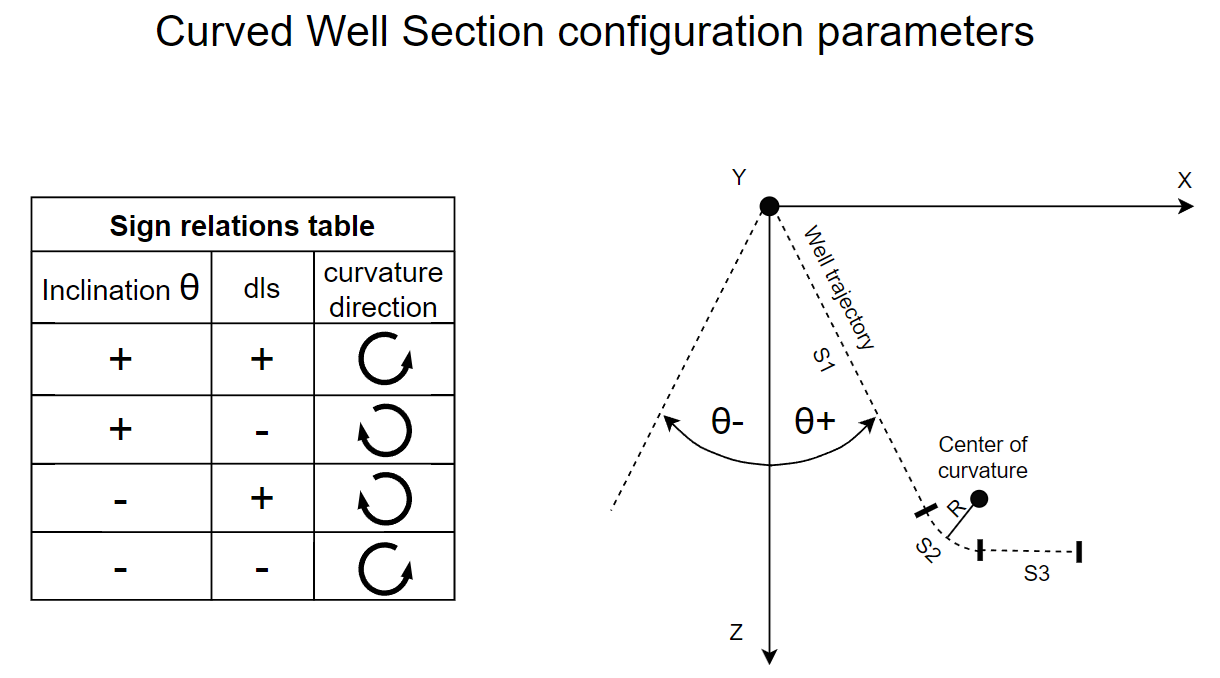
\includegraphics[width=1.0\textwidth]{"images/well_builder/dls_vs_inclination.png"}

	\subsection{IWellTemplate}
	\texttt{IWellTemplate} is a predefined section model consisting of one \texttt{LinearWellSection} with inclination equal to 0. In other words it is a vertical \texttt{LinearWellSection}. It is specified by following parameters:
	\begin{itemize}
		\item  \colorbox{gray!20}{name:} \texttt{str} - name of the well section.
		\item  \colorbox{gray!20}{wellhead:} \texttt{str} - starting position of the well section.
		\item  \colorbox{gray!20}{md:} \texttt{float} - the measured distance over the well section.
		\item  \colorbox{gray!20}{md\_step:} \texttt{float} - the sample distance over the segment's md. The parameter defines precision of the constructed well section discrete model.
		\item  \colorbox{gray!20}{perforations:} \texttt{Iterable[Perforation]} - optional perforations defined for the created well. Provided perforations are validated and returned with a well model.
	\end{itemize}
	\subsubsection{Methods}
	\begin{description}
		\item[\colorbox{gray!20}{from\_model}] \hfill
		\begin{description}
			\item arguments
		\begin{itemize}
			\item model: \texttt{IWellModel} - configuration model.
		\end{itemize}
		\item returns
			\begin{itemize}
				\item \texttt{IWellTemplate} - a object created with configuration provided in dedicated Pydantic model.
			\end{itemize}
		\end{description}
	\end{description}

\subsection{JWellTemplate}
\texttt{JWellTemplate} is a predefined section model consisting of two \texttt{LinearWellSection} objects and one \texttt{CurvedWellSection}:
\begin{itemize}
	\item  \colorbox{gray!20}{name:} \texttt{str} - name of the well section.
	\item  \colorbox{gray!20}{wellhead:} \texttt{str} - starting position of the well section.
	\item  \colorbox{gray!20}{azimuth:} \texttt{str} - rotation angle along z-axis of the well section.
	\item  \colorbox{gray!20}{md\_linear1:} \texttt{float} - the measured distance over the well section of the first \texttt{LinearWellSection}.
	\item  \colorbox{gray!20}{md\_curved:} \texttt{float} - the measured distance over the well section of the \texttt{CurvedWellSection}.
	\item  \colorbox{gray!20}{dls:} \texttt{float} - dogleg severity of the \texttt{CurvedWellSection}.
	\item  \colorbox{gray!20}{md\_linear2:} \texttt{float} - the measured distance over the well section of the second \texttt{LinearWellSection}.
	\item  \colorbox{gray!20}{md\_step:} \texttt{float} - the sample distance over the segment's md. The parameter defines precision of the constructed well section discrete model.
	\item  \colorbox{gray!20}{perforations:} \texttt{Iterable[Perforation]} - optional perforations defined for the created well. Provided perforations are validated and returned with a well model.
\end{itemize}
\subsubsection{Methods}
\begin{description}
	\item[\colorbox{gray!20}{from\_model}] \hfill
	\begin{description}
		\item arguments
		\begin{itemize}
			\item model: \texttt{JWellModel} - configuration model.
		\end{itemize}
		\item returns
		\begin{itemize}
			\item \texttt{JWellTemplate} - a object created with configuration provided in dedicated Pydantic model.
		\end{itemize}
	\end{description}
\end{description}

\subsection{SWellTemplate}
\texttt{SWellTemplate} is a predefined section model consisting of three \texttt{LinearWellSection} objects and two \texttt{CurvedWellSection} objects:
\begin{itemize}
	\item  \colorbox{gray!20}{name:} \texttt{str} - name of the well section.
	\item  \colorbox{gray!20}{wellhead:} \texttt{str} - starting position of the well section.
	\item  \colorbox{gray!20}{azimuth:} \texttt{str} - rotation angle along z-axis of the well section.
	\item  \colorbox{gray!20}{md\_linear1:} \texttt{float} - the measured distance over the well section of the first \texttt{LinearWellSection}.
	\item  \colorbox{gray!20}{md\_curved1:} \texttt{float} - the measured distance over the well section of the first \texttt{CurvedWellSection}.
	\item  \colorbox{gray!20}{dls1:} \texttt{float} - dogleg severity of the first \texttt{CurvedWellSection}.
	\item  \colorbox{gray!20}{md\_linear2:} \texttt{float} - the measured distance over the well section of the second \texttt{LinearWellSection}.
	\item  \colorbox{gray!20}{md\_curved2:} \texttt{float} - the measured distance over the well section of the second \texttt{CurvedWellSection}.
	\item  \colorbox{gray!20}{dls2:} \texttt{float} - dogleg severity of the second \texttt{CurvedWellSection}.
	\item  \colorbox{gray!20}{md\_linear3:} \texttt{float} - the measured distance over the well section of the third \texttt{LinearWellSection}.
	\item  \colorbox{gray!20}{md\_step:} \texttt{float} - the sample distance over the segment's md. The parameter defines precision of the constructed well section discrete model.
	\item  \colorbox{gray!20}{perforations:} \texttt{Iterable[Perforation]} - optional perforations defined for the created well. Provided perforations are validated and returned with a well model.
\end{itemize}
\subsubsection{Methods}
\begin{description}
	\item[\colorbox{gray!20}{from\_model}] \hfill
	\begin{description}
		\item arguments
		\begin{itemize}
			\item model: \texttt{SWellModel} - configuration model.
		\end{itemize}
		\item returns
		\begin{itemize}
			\item \texttt{SWellTemplate} - a object created with configuration provided in dedicated Pydantic model.
		\end{itemize}
	\end{description}
\end{description}

\subsection{HWellTemplate}
\texttt{JWellTemplate} is a predefined section model consisting of two \texttt{LinearWellSection} objects and one \texttt{CurvedWellSection}. The difference between this template and JWellTemplate is fixed DLS equal 4 [\textit{deg / 30m}] and curvature angle being always 90 [\textit{deg}].
\begin{itemize}
	\item  \colorbox{gray!20}{name:} \texttt{str} - name of the well section.
	\item  \colorbox{gray!20}{TVD:} \texttt{float} - \textit{true vertical depth} of the well starting from wellhead. The parameter includes first linear section and the depth build by curved well section.
	\item  \colorbox{gray!20}{md\_lateral:} \texttt{float} - total width of the well. The parameter includes second linear section and the width build by curved well section.
	\item  \colorbox{gray!20}{wellhead:} \texttt{TrajectoryPoint} - starting position of the first well section.
	\item  \colorbox{gray!20}{azimuth:} \texttt{float} - rotation angle along z-axis of the well section.
	\item  \colorbox{gray!20}{md\_step:} \texttt{float} - the sample distance over the segment's md. The parameter defines precision of the constructed well section discrete model.
	\item  \colorbox{gray!20}{perforations:} -  \texttt{Sequence[PerforationRange]} - collection of perforations defined by first perforated trajectory point md and the last perforated trajectory point md.

\end{itemize}
\subsubsection{Methods}
\begin{description}
	\item[\colorbox{gray!20}{from\_model}] \hfill
	\begin{description}
		\item arguments
		\begin{itemize}
			\item model: \texttt{HWellModel} - configuration model.
		\end{itemize}
		\item returns
		\begin{itemize}
			\item \texttt{HWellTemplate} - a object created with configuration provided in dedicated Pydantic model.
		\end{itemize}
	\end{description}
\end{description}

\subsection{WellBuilder}
	\texttt{WellBuilder} is a class responsible for integrating each well sections into one coherent part. Thanks to this class we can manipulate the overall structure of the bore by translating and rotating the whole structure. \textbf{Please note that all methods regarding this class are being applied in place.}
	WellBuilder calls building method for each well section and collects resulted points in one \textit{Trajectory} object. This process was visualized in the following figure:\\\\
	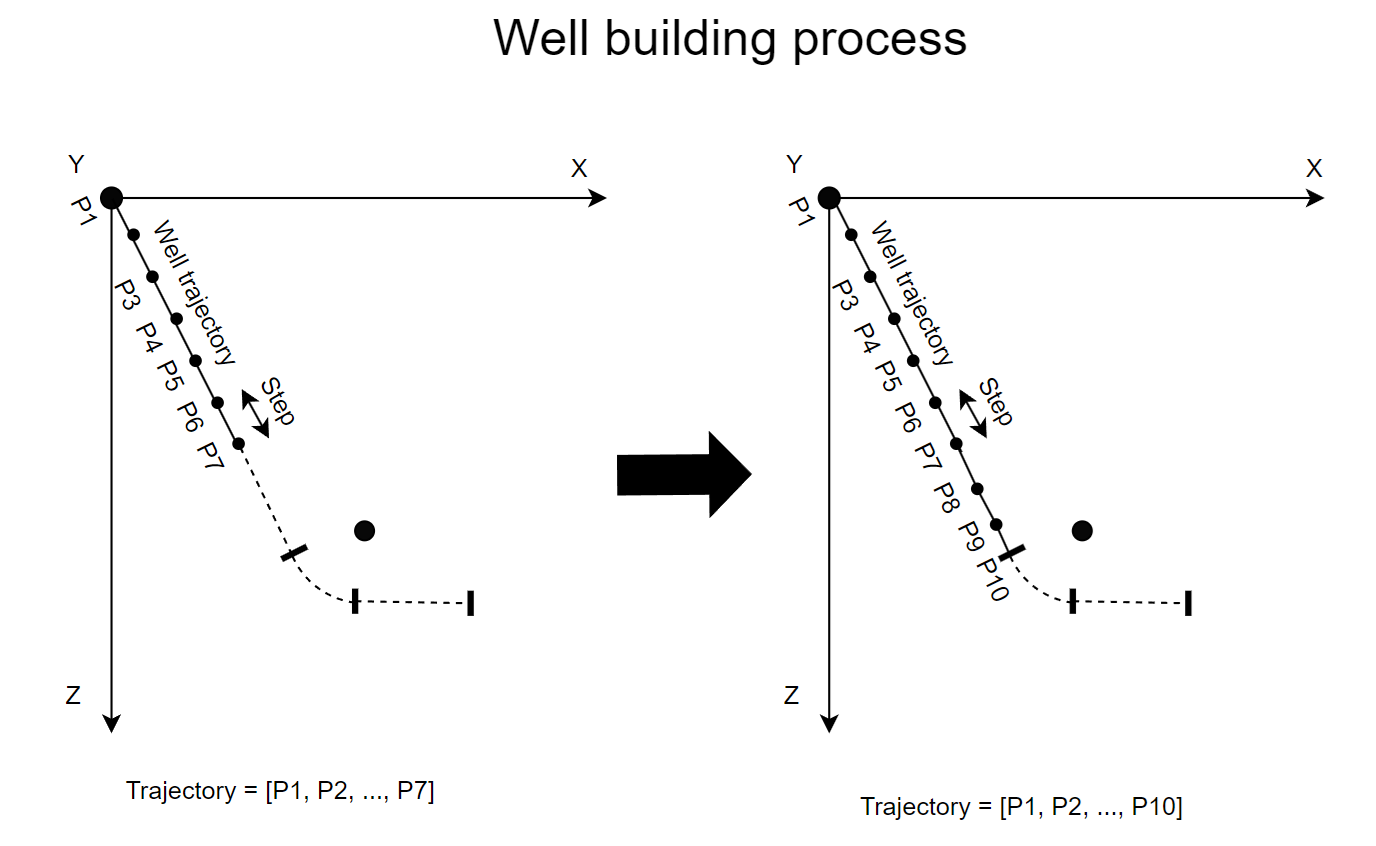
\includegraphics[width=\textwidth]{"images/well_builder/well_building_process.png"}\\

	\subsubsection{Methods}
	\begin{description}

		\item[ \colorbox{gray!20}{well\_name}] \hfill
		\begin{description}
			\item[Arguments:] \hfill
			\begin{itemize}
				\item \texttt{name} (\texttt{str}) - name which we want to call our well.
			\end{itemize}
			\item[Returns:] \hfill
			\begin{itemize}
				\item \texttt{WellBuilder} - instance of this class with modified name.
			\end{itemize}
		\end{description}

		\item[ \colorbox{gray!20}{rotate}] \hfill
		\begin{description}
			\item[Arguments:] \hfill
			\begin{itemize}
				\item \texttt{azimuth} (\texttt{float}) - the azimuth angle in degrees to rotate the well.
			\end{itemize}
			\item[Returns:] \hfill
			\begin{itemize}
				\item \texttt{WellBuilder} - instance of this class with the modified azimuth.
			\end{itemize}
		\end{description}

		\item[ \colorbox{gray!20}{translate}] \hfill
		\begin{description}
			\item[Arguments:] \hfill
			\begin{itemize}
				\item \texttt{translation} (\texttt{Vector}) - the vector by which the well should be translated.
			\end{itemize}
			\item[Returns:] \hfill
			\begin{itemize}
				\item \texttt{WellBuilder} - instance of this class with the modified translation.
			\end{itemize}
		\end{description}

		\item[ \colorbox{gray!20}{discretize}] \hfill
		\begin{description}
			\item[Arguments:] \hfill
			\begin{itemize}
				\item \texttt{step} (\texttt{float}) - the step size for trajectory discretization in meters.
			\end{itemize}
			\item[Returns:] \hfill
			\begin{itemize}
				\item \texttt{WellBuilder} - instance of this class with the modified discretization step.
			\end{itemize}
		\end{description}

		\item[ \colorbox{gray!20}{sections}] \hfill
		\begin{description}
			\item[Arguments:] \hfill
			\begin{itemize}
				\item \texttt{sections} (\texttt{Iterable[SectionInterface]}) - collection of sections to define the well structure.
			\end{itemize}
			\item[Returns:] \hfill
			\begin{itemize}
				\item \texttt{WellBuilder} - instance of this class with the modified well sections.
			\end{itemize}
		\end{description}

		\item[ \colorbox{gray!20}{perforations}] \hfill
		\begin{description}
			\item[Arguments:] \hfill
			\begin{itemize}
				\item \texttt{perforations} (\texttt{Iterable[Perforation]}) - collection of perforations defined as measured distance ranges within the trajectory.
			\end{itemize}
			\item[Returns:] \hfill
			\begin{itemize}
				\item \texttt{WellBuilder} - instance of this class with the modified perforations.
			\end{itemize}
		\end{description}

		\item[ \colorbox{gray!20}{build}] \hfill
		\begin{description}
			\item[Description:] \hfill
			\begin{itemize}
				\item This method builds the well's trajectory by combining all defined sections, applying rotation and translation to the trajectory.
			\end{itemize}

			\item[Returns:] \hfill
			\begin{itemize}
				\item \texttt{Well} - the final well model after applying all sections, rotation, translation and additional information like perforations.
			\end{itemize}

			\item[Raises:] \hfill
			\begin{itemize}
				\item \texttt{EmptySegmentConfigurationException} - if the well builder has no valid sections configuration.
			\end{itemize}
		\end{description}

	\end{description}
